\documentclass[aspectratio=169,11pt]{beamer}
\usepackage[T1]{fontenc}
\usepackage{booktabs,tabularx,amsmath,amssymb,tikz}
\usetikzlibrary{positioning,arrows.meta,fit,shapes.misc}
\graphicspath{{figures/}{../thesis/figures/}}

% ---------------------------------------------------------------- look
\definecolor{navy}{HTML}{1B2A4A}
\definecolor{teal}{HTML}{0E7271}
\definecolor{tealbg}{HTML}{E8F3F2}
\definecolor{maroon}{HTML}{9C1D55}
\definecolor{alertred}{HTML}{C62828}
\definecolor{softgrey}{HTML}{6B7280}

\setbeamertemplate{navigation symbols}{}
\setbeamercolor{structure}{fg=maroon}
\setbeamercolor{normal text}{fg=black}
\setbeamercolor{alerted text}{fg=alertred}
\setbeamercolor{block title}{bg=teal,fg=white}
\setbeamercolor{block body}{bg=tealbg,fg=black}
\setbeamercolor{block title alerted}{bg=white,fg=alertred}
\setbeamercolor{block body alerted}{bg=white,fg=black}
\setbeamerfont{block title}{size=\normalsize}
\setbeamertemplate{blocks}[default]
\setbeamertemplate{enumerate items}[default]
\setbeamertemplate{itemize items}[circle]
\setbeamercolor{enumerate item}{fg=maroon}
\setbeamercolor{itemize item}{fg=navy}

\setbeamertemplate{frametitle}{%
  \nointerlineskip
  \begin{beamercolorbox}[wd=\paperwidth,ht=2.6ex,dp=1.4ex,leftskip=1.2em]{frametitle}
    \usebeamerfont{frametitle}\insertframetitle
  \end{beamercolorbox}}
\setbeamercolor{frametitle}{bg=navy,fg=white}
\setbeamerfont{frametitle}{size=\Large}
\setbeamertemplate{footline}{%
  \hfill\usebeamercolor[fg]{normal text}\scriptsize\insertframenumber\,/\,\inserttotalframenumber\hspace*{1.2em}\vspace*{0.8em}}

\newcommand{\finding}[2]{\par\vspace{0.5em}{\color{alertred}\large #1}\par\smallskip #2\par}
\newcolumntype{Y}{>{\raggedright\arraybackslash}X}
\newcommand{\src}[1]{\par\vspace{0.2em}{\tiny\color{softgrey}#1}}

\title{CardioCog: An Explainable AI Framework for Cognitive Health Assessment and Early Prediction of Cognitive Decline Using Cardiovascular, Genetic, and Clinical Factors}

\begin{document}

% ================================================================ title
{\setbeamertemplate{footline}{}
\begin{frame}[noframenumbering]
\centering
\vspace{0.6em}
{\color{maroon}\bfseries\large CardioCog: An Explainable AI Framework for Cognitive Health Assessment and Early Prediction of Cognitive Decline Using Cardiovascular, Genetic, and Clinical Factors\par}
\vspace{1.0em}
FINAL REVIEW -- B.TECH PROJECT\par
\vspace{0.8em}
Team No.: D07\par
\vspace{0.5em}
\small
\begin{tabular}{ll}
Akula Akhil Vighnesh & CB.SC.U4AIE23303 \\
Vada Gouri Hansika Reddy & CB.SC.U4AIE23304 \\
Pilli Venkata Bhargav Reddy & CB.SC.U4AIE23329 \\
Marella Venkata Mahidhar Reddy & CB.SC.U4AIE23354 \\
\end{tabular}\par
\vspace{0.8em}
\normalsize Supervisor: Dr.\ Manoj Bhat K, Professor\par
\vspace{0.8em}
AMRITA VISHWA VIDYAPEETHAM -- SCHOOL OF ARTIFICIAL INTELLIGENCE, COIMBATORE
\end{frame}}

% ================================================================ 01 progress
\begin{frame}{01 \textbar\ Research Progress: From Proposal to Evidence}
\begin{block}{Research progression}
Zeroth review: multimodal framework $\rightarrow$ first review: 3D amyloid-PET prototype (198 people, 17 events) $\rightarrow$ full NACC clinical cohort (19,470 people, 2,818 events) $\rightarrow$ two decline outcomes, five models, fusion network $\rightarrow$ PET image pipeline, prototype, 17 verification checks.
\end{block}
\footnotesize
\begin{tabularx}{\textwidth}{@{}lY@{}}
\toprule
\textbf{Milestone} & \textbf{Evidence and outcome} \\
\midrule
First-review prototype & 3D CNN + cross-attention on amyloid PET: AUROC 0.786 in one run, 0.652 on re-run. Too few events to conclude. \\
Leakage-free cohort & First visit, not demented, UDS v1--3; person-level split with 9 whole centres held out. \\
Dementia in 3 years & XGBoost AUROC 0.938 (test), 0.946 (held-out centres); 0.84 within MCI. \\
Cognitive decline & CDR-SB rise $\geq 1$: AUROC 0.858 / 0.885; CDR-SB change regression helps MCI. \\
Independent checks & 17 of 17 checks pass; two future-information errors found and fixed. \\
\bottomrule
\end{tabularx}
\end{frame}

% ================================================================ 02 problem
\begin{frame}{02 \textbar\ Motivation and Problem Statement}
\small
\begin{block}{Problem}
Clinics already record cognition, vascular history, genetics and sometimes PET for older adults without dementia, but rarely combine them into one \emph{explainable} estimate of near-term decline. Which of these sources actually adds information, and can the estimate be trusted?
\end{block}
\vspace{0.3em}
For a person without dementia at visit $t_0$, estimate over the next three years:
\[
\hat{p}_{\text{dem}} = P(\text{dementia} \mid \mathbf{x}_{t_0}), \quad
\hat{p}_{\text{dec}} = P(\Delta\text{CDR-SB} \geq 1 \mid \mathbf{x}_{t_0}), \quad
\hat{\Delta} = E(\Delta\text{CDR-SB} \mid \mathbf{x}_{t_0})
\]
\footnotesize
\begin{enumerate}
\setlength{\itemsep}{0pt}
\item How accurately can both outcomes be predicted, for normal and MCI groups separately?
\item Does cardiovascular history add to demographics, genetics and current cognition?
\item Do amyloid and tau PET add to the clinical model?
\item Do deep models, including a modality-encoder fusion network, beat classical ones?
\item Do earlier visits help? \qquad 6.\ Can one model cope with missing categories? \qquad 7.\ Can each estimate be explained with evidence?
\end{enumerate}
\end{frame}

% ================================================================ 03 literature
\begin{frame}{03 \textbar\ Literature Review and Research Gap}
\scriptsize
\begin{tabularx}{\textwidth}{@{}p{3.1cm}p{4.2cm}Y@{}}
\toprule
Work & Core method & Relevance / limitation for CardioCog \\
\midrule
Livingston et al.\ (2020) & Lancet Commission, 12 modifiable risk factors & Vascular risk matters over the life course; mostly midlife exposure \\
Alaka et al.\ (2025) & CAIDE + heart rate, random forest, NACC & Same database; AUC 0.80--0.91, no within-stage results \\
Stern \& Linial (2026) & CatBoost on UK Biobank codes + APOE & AUROC 0.773 without cognitive inputs \\
Aschwanden et al.\ (2020) & Random survival forests, 52 predictors & Cardiovascular factors less important than expected \\
Yi et al.\ (2023) & XGBoost + SHAP for diagnosis & CDR-SB most important; diagnosis, not prediction \\
Gorishniy et al.\ (2021) & FT-Transformer for tabular data & No deep model consistently beats boosted trees \\
Lewis et al.\ (2020) & Retrieval-augmented generation & Grounds generated text in a fixed library \\
\bottomrule
\end{tabularx}
\begin{block}{Research gap}
\small Few studies measure, on one large leakage-controlled cohort, \textbf{how much each source adds once current cognition is known}, with results \textbf{within} normal and MCI groups.
\end{block}
\end{frame}

% ================================================================ first review
\begin{frame}{Why the design changed after the first review}
\begin{columns}[T]
\begin{column}{0.48\textwidth}
\begin{block}{First-review prototype}
3D CNN on raw amyloid PET + 34 clinical features, spatial cross-attention, 1-year CDR-SB rise $\geq 0.5$.
\end{block}
\small
\begin{tabular}{@{}lc@{}}
\toprule
Run & Mean AUROC (SD) \\
\midrule
Reported at review & 0.786 (0.134) \\
Re-run, same notebook & 0.652 (0.153) \\
\bottomrule
\end{tabular}
\end{column}
\begin{column}{0.48\textwidth}
\finding{Diagnosis}{Only 198 people and \textbf{17 events}: a handful of participants decides the score. The pipeline also mixed PET time frames, had no registration, read one non-existent column and fitted SHAP on all data.}
\finding{Decision}{Move to the full clinical cohort with three-year outcomes and thousands of events; treat PET images as a separate, validated pipeline.}
\end{column}
\end{columns}
\end{frame}

% ================================================================ 04 data
\begin{frame}{04 \textbar\ Data: NACC Freeze 74 and the Cohort}
\begin{columns}[T]
\begin{column}{0.47\textwidth}
\footnotesize
\begin{tabular}{@{}lr@{}}
\toprule
Step & Participants \\
\midrule
All participants & 57,038 \\
First visit, in person, UDS v1--3 & 55,461 \\
\quad not demented at that visit & 38,107 \\
\quad outcome known at 3 years & 19,470 \\
\quad\quad converted to dementia & 2,818 (14.5\%) \\
\bottomrule
\end{tabular}
\vspace{0.5em}
\begin{block}{Three groups, very different risk}
Normal 12,377 (1.6\% convert) \\ MCI 5,993 (41.5\%) \\ Impaired, not MCI 1,100 (12.3\%)
\end{block}
\end{column}
\begin{column}{0.5\textwidth}
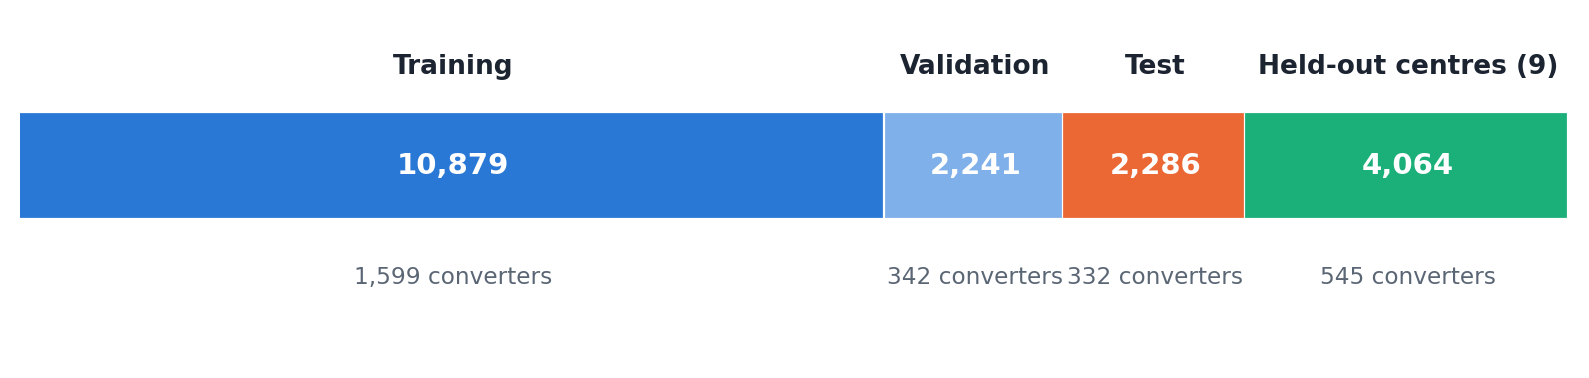
\includegraphics[width=\textwidth]{split.png}
\small
\begin{itemize}
\item Person-level split; \textbf{9 of 46 centres held out} entirely.
\item Train 70\% / validation 15\% / test 15\%, seed 2026.
\item Every normaliser and imputer fitted on training data only.
\end{itemize}
\end{column}
\end{columns}
\end{frame}

% ================================================================ outcome
\begin{frame}{Outcomes and censoring}
\begin{columns}[c]
\begin{column}{0.55\textwidth}
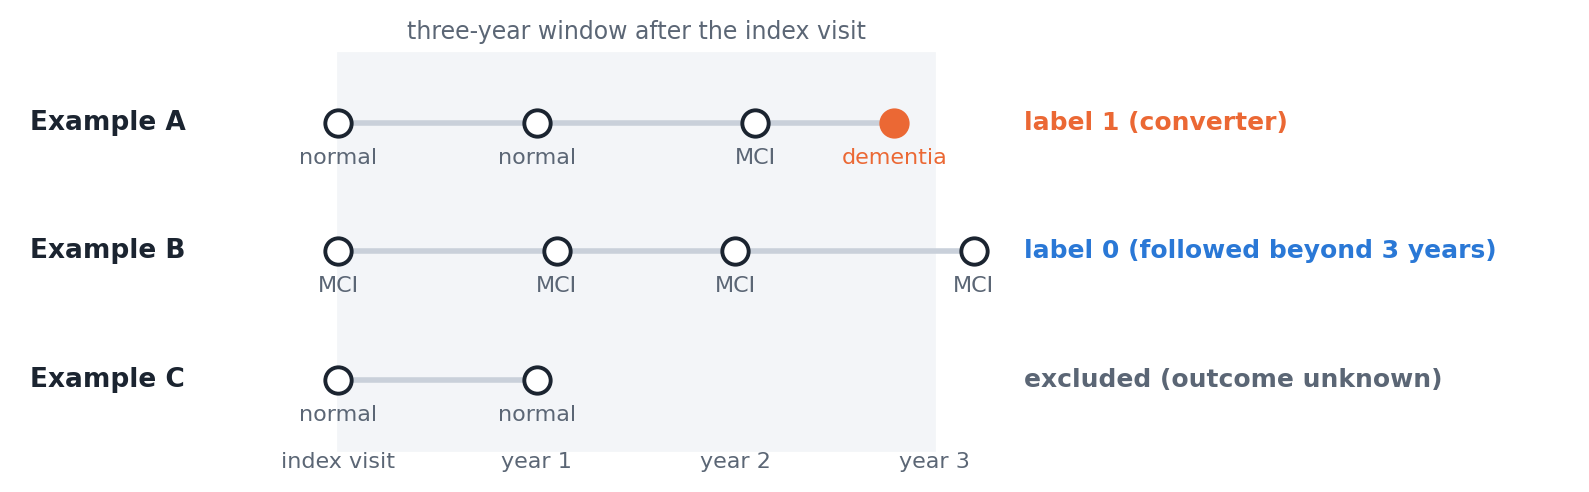
\includegraphics[width=\textwidth]{outcome.png}
\end{column}
\begin{column}{0.43\textwidth}
\small
\[
y = \begin{cases} 1 & T \le 3 \\ 0 & T > 3,\ C \ge 3 \\ \text{unknown} & T > 3,\ C < 3 \end{cases}
\]
$T$: years to dementia diagnosis, $C$: years to last visit.
\begin{block}{Secondary outcomes}
CDR-SB rise $\geq 1$ within 3 years (20,355 people, 5,035 events) and the 3-year change $\Delta$ in CDR-SB.
\end{block}
\finding{Robustness}{A Cox model that keeps censored participants gives the same conclusions.}
\end{column}
\end{columns}
\end{frame}

% ================================================================ 05 features
\begin{frame}{05 \textbar\ 48 Features in Five Categories}
\begin{columns}[T]
\begin{column}{0.48\textwidth}
\small
\begin{tabular}{@{}lc@{}}
\toprule
Category & Features \\
\midrule
Demographics & 8 \\
Cardiovascular and medical & 25 \\
Cognitive tests ($z$-scores) & 9 \\
Clinical stage (CDR-SB, diagnosis) & 3 \\
Genetics (APOE $\varepsilon$4, family history) & 3 \\
PET (second-stage model only) & 4 \\
\bottomrule
\end{tabular}
\begin{block}{Harmonising tests across form versions}
\[
\hat{s} = \beta_0 + \beta_1\,\text{age} + \beta_2\,\text{female} + \beta_3\,\text{educ}
\]
\[
z = (s - \hat{s}) / \sigma_{\text{res}}
\]
Fitted on cognitively normal training participants.
\end{block}
\end{column}
\begin{column}{0.5\textwidth}
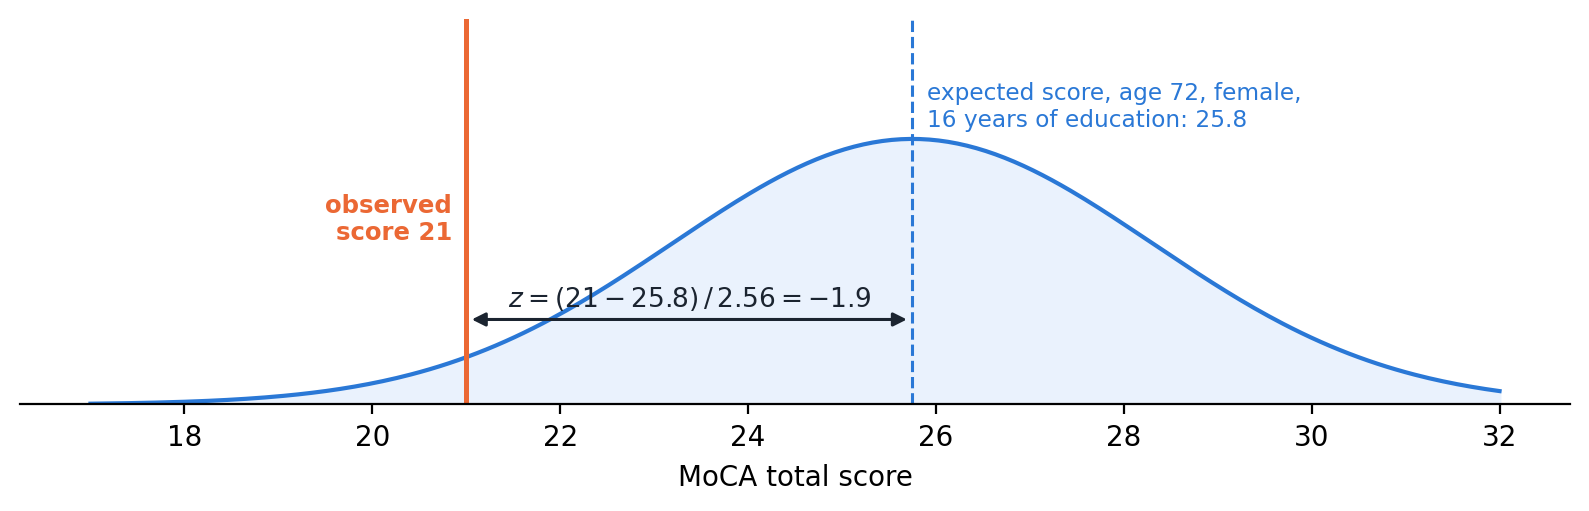
\includegraphics[width=\textwidth]{zscore.png}
\small MoCA example: expected 25.8 for a 72-year-old woman with 16 years of education, so a score of 21 gives $z = -1.9$. Healthy people not used for fitting score within 0.1 of zero in every UDS version.
\end{column}
\end{columns}
\end{frame}

% ================================================================ pipeline
\begin{frame}{06 \textbar\ Methodology: the CardioCog Pipeline}
\centering
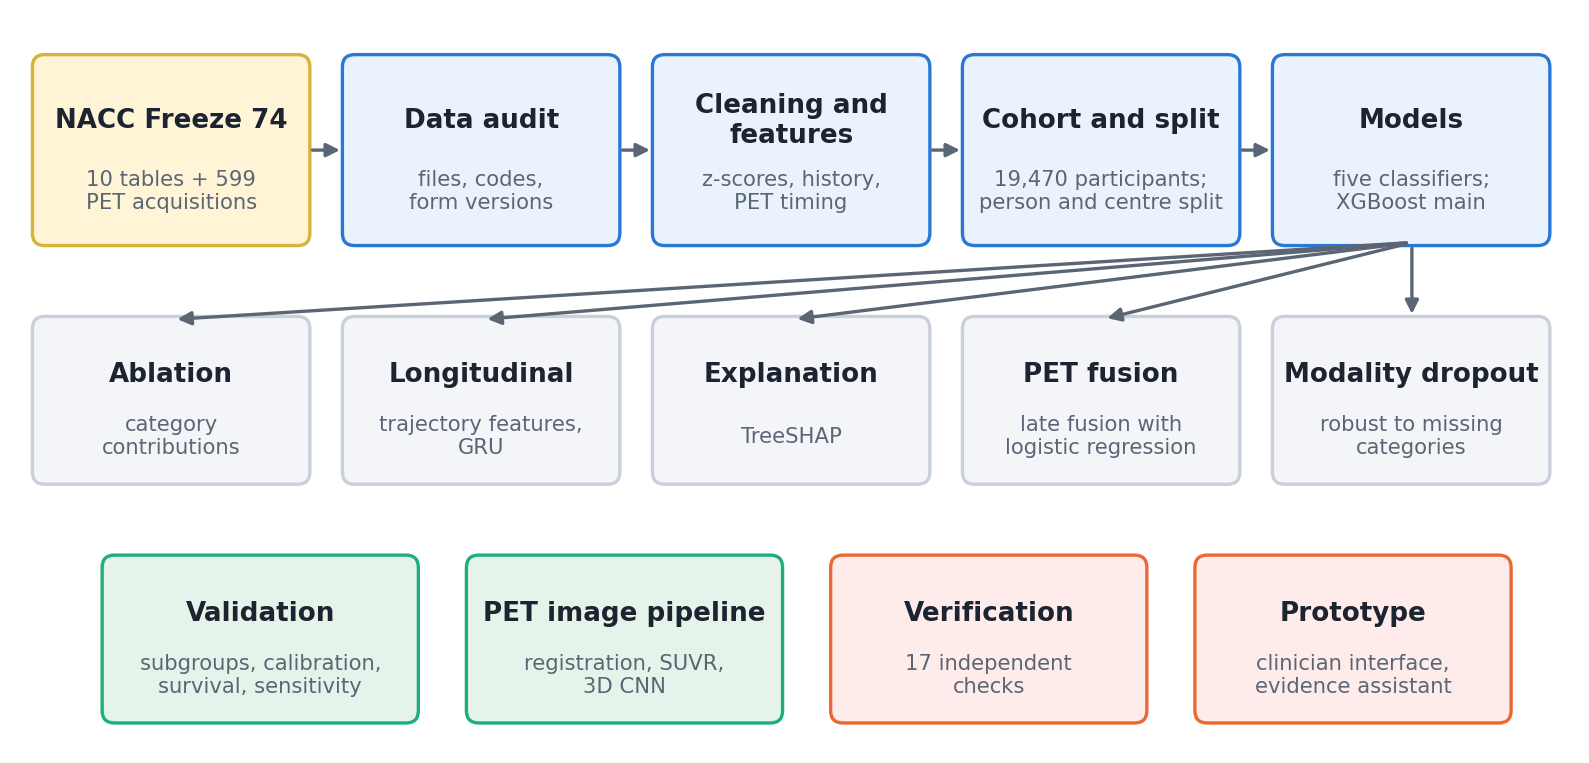
\includegraphics[width=0.8\textwidth]{pipeline.png}
\small
\begin{block}{Rule for every step}
Only information available at the index visit; anything learned from data is fitted on the training set; results are reported on the test set and on centres never seen in training.
\end{block}
\end{frame}

% ================================================================ models
\begin{frame}{Models compared on the same 48 features}
\begin{columns}[T]
\begin{column}{0.5\textwidth}
\small
\begin{tabularx}{\textwidth}{@{}lY@{}}
\toprule
Model & Key settings \\
\midrule
Logistic regression & $L_2$, $C$ from 5 values \\
Random forest & 500 trees, $\sqrt{p}$ features \\
XGBoost & $\eta = 0.03$, depth 3--6, $\lambda = 2$, early stop \\
MLP & 128--64 units, dropout 0.2 \\
FT-Transformer & 64-d tokens, 3 layers, 8 heads \\
\bottomrule
\end{tabularx}
\vspace{0.3em}
Three seeds averaged; XGBoost chosen as the main model (handles missing values, exact SHAP).
\end{column}
\begin{column}{0.48\textwidth}
\small
\begin{block}{XGBoost objective}
\[
f_M(\mathbf{x}) = \sum_{m=1}^{M} \eta\, g_m(\mathbf{x}),
\quad
w_j^{*} = -\frac{\sum_{i \in I_j} G_i}{\sum_{i \in I_j} H_i + \lambda}
\]
\end{block}
\begin{block}{Loss and evaluation}
\[
\mathcal{L}_{\text{BCE}} = -\tfrac{1}{n}\textstyle\sum_i \big[y_i \log \hat{p}_i + (1-y_i)\log(1-\hat{p}_i)\big]
\]
AUROC, AUPRC, Brier, calibration slope, net benefit; 1,000 paired bootstrap resamples.
\end{block}
\end{column}
\end{columns}
\end{frame}

% ================================================================ fusion network
\begin{frame}{Modality-encoder fusion network (proposed architecture)}
\centering
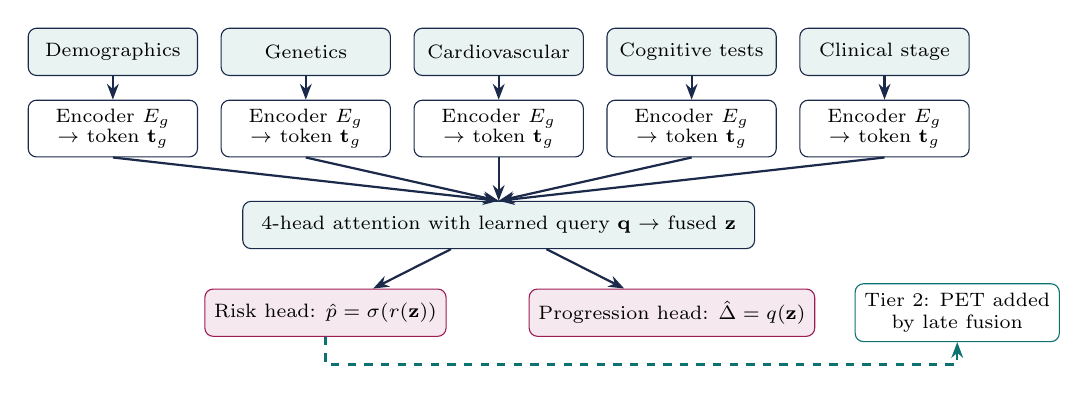
\begin{tikzpicture}[
  box/.style={draw=navy, rounded corners=3pt, fill=tealbg, minimum width=2.15cm, minimum height=0.6cm, font=\scriptsize, align=center},
  enc/.style={box, fill=white},
  head/.style={box, fill=maroon!10, draw=maroon, minimum width=2.8cm},
  arr/.style={-{Stealth[length=2mm]}, navy, thick}]
\foreach \name/\lab [count=\i] in {d/Demographics, g/Genetics, c/Cardiovascular, t/Cognitive tests, s/Clinical stage} {
  \node[box] (in\name) at (\i*2.45, 0) {\lab};
  \node[enc, below=0.3cm of in\name] (e\name) {Encoder $E_g$\\[-1pt] $\rightarrow$ token $\mathbf{t}_g$};
  \draw[arr] (in\name) -- (e\name);
}
\node[box, minimum width=6.5cm, below=0.55cm of ec] (att) {4-head attention with learned query $\mathbf{q}$ $\rightarrow$ fused $\mathbf{z}$};
\foreach \name in {d,g,c,t,s} \draw[arr] (e\name.south) -- (att.north);
\node[head, below=0.5cm of att, xshift=-2.2cm] (risk) {Risk head: $\hat{p} = \sigma(r(\mathbf{z}))$};
\node[head, below=0.5cm of att, xshift=2.2cm] (prog) {Progression head: $\hat{\Delta} = q(\mathbf{z})$};
\draw[arr] (att) -- (risk); \draw[arr] (att) -- (prog);
\node[box, fill=white, draw=teal, right=0.5cm of prog] (pet) {Tier 2: PET added\\ by late fusion};
\draw[arr, teal, dashed] (risk.south) |- ++(0,-0.35) -| (pet.south);
\end{tikzpicture}

\vspace{0.2em}
\footnotesize A missing modality gets a learned token $\mathbf{m}_g$; each token gets a type embedding $\boldsymbol{\tau}_g$; whole modalities are hidden with probability 0.35 in training.
\small
\[
\mathcal{L} = \mathcal{L}_{\text{BCE}} + 0.5\cdot\text{Huber}(\Delta - \hat{\Delta}), \qquad
\alpha_g = \operatorname{softmax}_g\!\big((\mathbf{W}_Q\mathbf{q})^{\top}\mathbf{W}_K\mathbf{t}_g/\sqrt{8}\big)
\]
\end{frame}

% ================================================================ 07 results models
\begin{frame}{07 \textbar\ Results: Dementia Within Three Years}
\small
\begin{tabular}{@{}lccccc@{}}
\toprule
 & \multicolumn{3}{c}{Test set (2,286 / 332 events)} & \multicolumn{2}{c}{Held-out centres (4,064 / 545)} \\
\cmidrule(lr){2-4}\cmidrule(l){5-6}
Model & AUROC (95\% CI) & AUPRC & Brier & AUROC & Brier \\
\midrule
Logistic regression & 0.936 (0.924--0.949) & 0.721 & 0.066 & 0.945 & 0.060 \\
Random forest & 0.932 (0.919--0.944) & 0.704 & 0.070 & 0.940 & 0.064 \\
XGBoost & \textbf{0.938} (0.925--0.948) & 0.713 & 0.066 & \textbf{0.946} & 0.059 \\
MLP & 0.938 (0.926--0.949) & 0.721 & 0.066 & 0.946 & 0.059 \\
FT-Transformer & 0.939 (0.927--0.949) & 0.720 & 0.066 & 0.945 & 0.061 \\
\bottomrule
\end{tabular}
\begin{block}{What the result does establish}
All five models discriminate well and are well calibrated (constant-prediction Brier 0.124), at new centres as well as on the test set.
\end{block}
\begin{block}{What it does not establish}
Intervals overlap almost completely: deep models give \textbf{no gain} over logistic regression or boosted trees.
\end{block}
\end{frame}

% ================================================================ by group
\begin{frame}{Is 0.94 too good? Results within diagnostic groups}
\begin{columns}[T]
\begin{column}{0.52\textwidth}
\small
\begin{tabular}{@{}lcc@{}}
\toprule
Group (test / held-out) & Test & Held-out \\
\midrule
All not demented & 0.937 & 0.946 \\
Cognitively normal (24 / 37 ev.) & 0.884 & 0.876 \\
MCI (289 / 496 ev.) & 0.835 & 0.846 \\
\bottomrule
\end{tabular}
\vspace{0.5em}
\begin{block}{Interpretation}
Diagnosis alone gives AUROC 0.84, because MCI converts 25 times as often as normal cognition. Within MCI the model still ranks risk at \textbf{0.84}.
\end{block}
\end{column}
\begin{column}{0.46\textwidth}
\finding{Critical check}{Removing \emph{all} current-cognition information drops AUROC from 0.937 to \textbf{0.746}.}
\finding{Meaning}{The model estimates short-term progression \emph{given} the current clinical stage. It is not leakage: inputs are from the index visit, the label from later visits.}
\end{column}
\end{columns}
\end{frame}

% ================================================================ ablation
\begin{frame}{What drives the prediction? Category ablation}
\centering
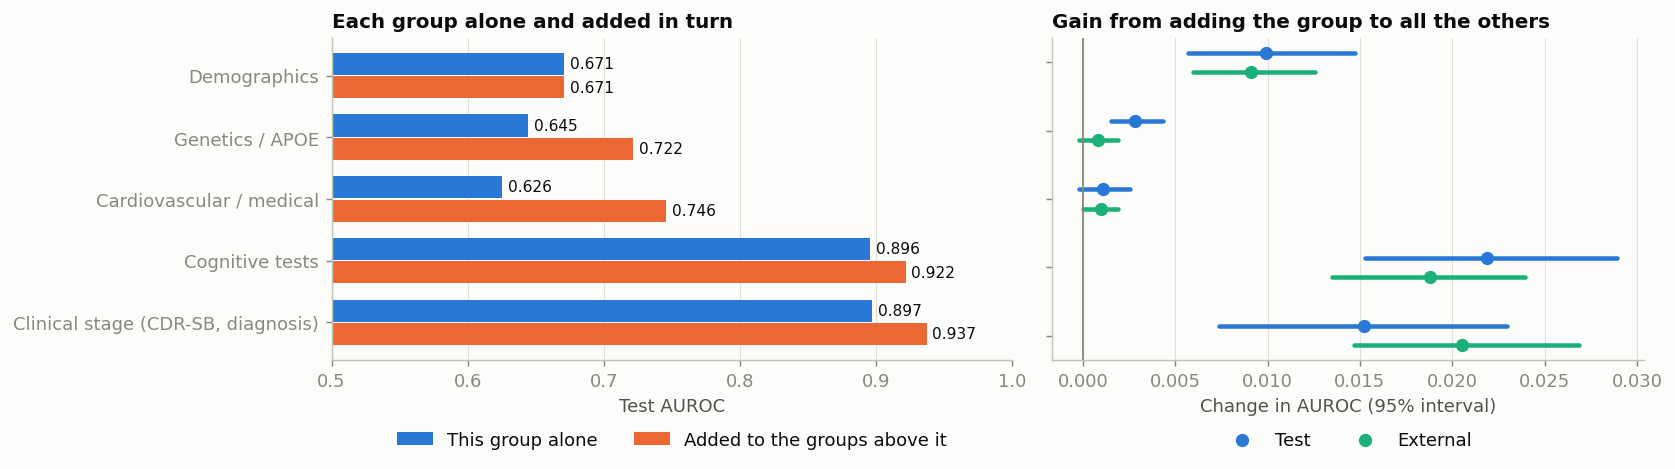
\includegraphics[width=0.92\textwidth]{06_feature_groups.png}
\small
\begin{tabular}{@{}lccc@{}}
\toprule
Category & Alone & Gain added last (test) & Gain (held-out) \\
\midrule
Cognitive tests & 0.896 & $+0.022$ & $+0.019$ \\
Clinical stage & 0.897 & $+0.015$ & $+0.021$ \\
Demographics & 0.671 & $+0.010$ & $+0.009$ \\
Genetics (APOE) & 0.645 & $+0.003$ & $+0.001$ \\
Cardiovascular / medical & 0.626 & $+0.001$ & $+0.001$ \\
\bottomrule
\end{tabular}
\end{frame}

% ================================================================ cardio
\begin{frame}{The cardiovascular question (RQ2)}
\begin{columns}[c]
\begin{column}{0.5\textwidth}
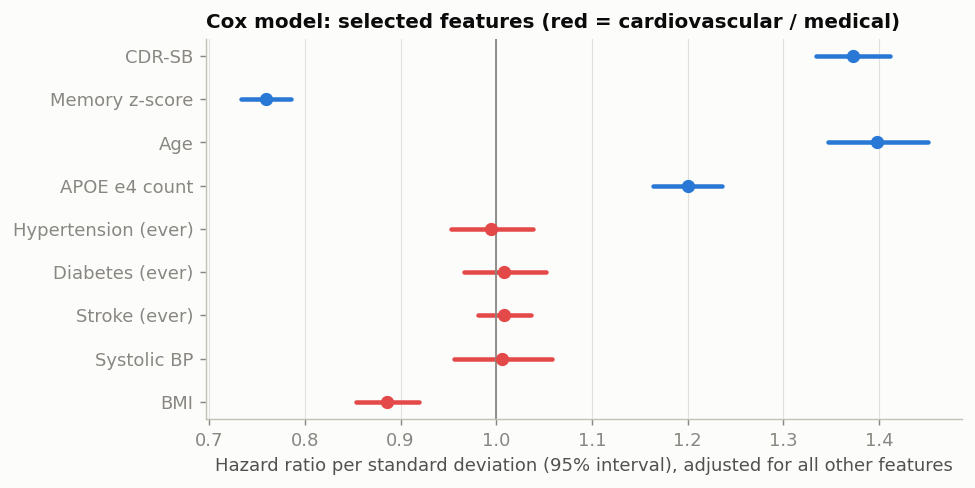
\includegraphics[width=\textwidth]{09_hazard_ratios.png}
\end{column}
\begin{column}{0.48\textwidth}
\small
\begin{itemize}
\item Alone: AUROC \textbf{0.626}; before cognition: $+0.024$ (test), $+0.004$ (held-out).
\item After cognition: $+0.001$ for dementia, $+0.0004$ for CDR-SB decline.
\item Cox model: hypertension HR 0.995, diabetes and stroke $\approx 1$.
\end{itemize}
\begin{block}{Interpretation}
Limited \emph{incremental} value in this cohort, not evidence that vascular health is unimportant: median age 71, midlife exposure unobserved, and past damage already shows in the cognitive scores.
\end{block}
\end{column}
\end{columns}
\end{frame}

% ================================================================ shap
\begin{frame}{Explainability: Shapley values}
\begin{columns}[c]
\begin{column}{0.58\textwidth}
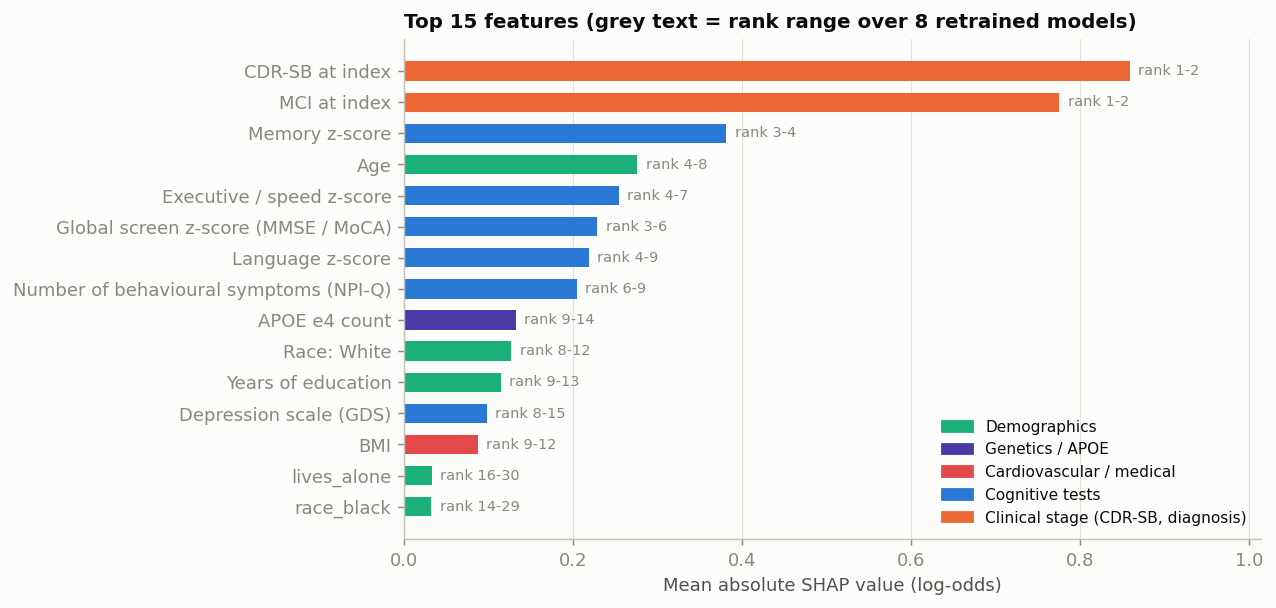
\includegraphics[width=\textwidth]{07_shap_features.png}
\end{column}
\begin{column}{0.4\textwidth}
\small
\[
f(\mathbf{x}) = \phi_0 + \sum_{j} \phi_j
\]
\begin{tabular}{@{}lc@{}}
\toprule
Category & SHAP share \\
\midrule
Clinical stage & 40.8\% \\
Cognitive tests & 35.0\% \\
Demographics & 15.5\% \\
Cardiovascular & 5.1\% \\
Genetics & 3.5\% \\
\bottomrule
\end{tabular}
\par\vspace{0.4em}
Stable over 8 refits (Spearman 0.89--0.97). Low BMI raises risk: weight loss before diagnosis, not causal.
\end{column}
\end{columns}
\end{frame}

% ================================================================ decline
\begin{frame}{Cognitive decline as the outcome}
\centering
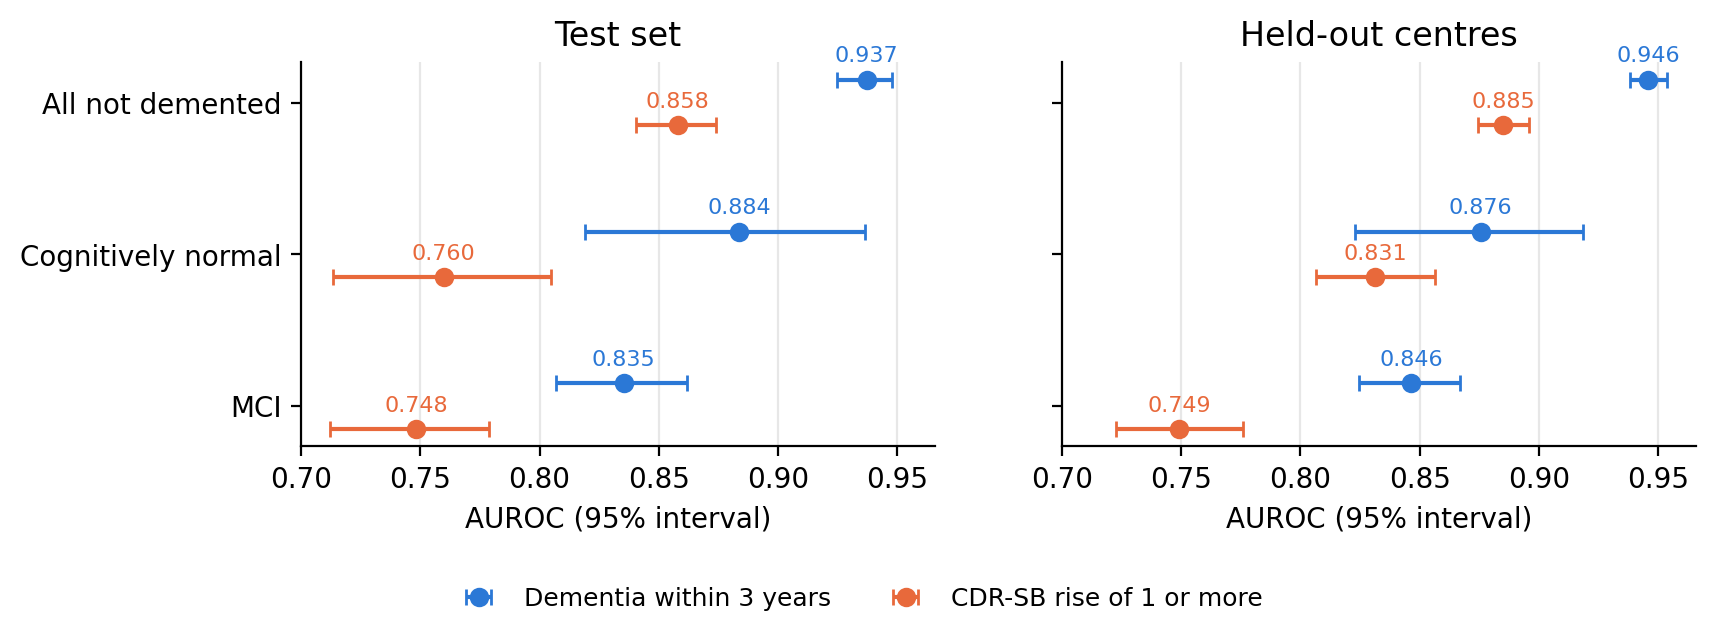
\includegraphics[width=0.82\textwidth]{decline_vs_dementia.png}
\begin{columns}[T]
\begin{column}{0.49\textwidth}
\begin{block}{CDR-SB rise $\geq 1$ (20,355 / 5,035 events)}
\small AUROC 0.858 test, 0.885 held-out; normal 0.76--0.83 with 129 and 215 events, so more reliable than the dementia estimate for normal cognition.
\end{block}
\end{column}
\begin{column}{0.49\textwidth}
\begin{block}{Predicted 3-year CDR-SB change}
\small MAE 0.69 $\rightarrow$ 0.60 (test), 0.82 $\rightarrow$ 0.72 (held-out); MCI 1.90 $\rightarrow$ 1.59; normal 0.17 = 0.17, no gain.
\end{block}
\end{column}
\end{columns}
\end{frame}

% ================================================================ fusion results
\begin{frame}{Fusion network: works, but no gain and uninformative attention}
\begin{columns}[c]
\begin{column}{0.56\textwidth}
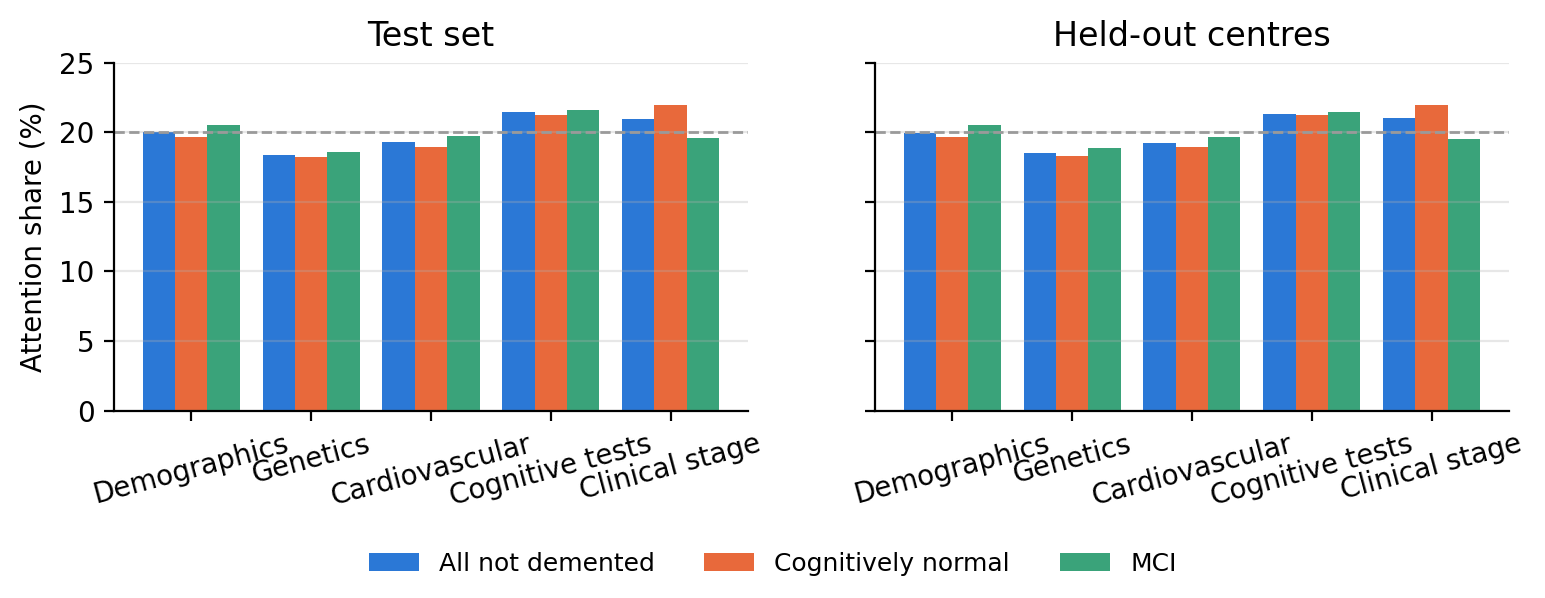
\includegraphics[width=\textwidth]{fusion_attention.png}
\end{column}
\begin{column}{0.42\textwidth}
\small
\begin{tabular}{@{}lcc@{}}
\toprule
AUROC & Fusion net & XGBoost \\
\midrule
Test & 0.934 & 0.937 \\
Held-out & 0.943 & 0.946 \\
MCI (test) & 0.831 & 0.835 \\
\bottomrule
\end{tabular}
\vspace{0.3em}

Progression head MAE 0.72 $\rightarrow$ 0.65. Without cognition: AUROC 0.72, Brier 0.114.
\finding{Finding}{Attention is 18--22\% for every modality (uniform = 20\%), so it does not explain predictions. SHAP and ablation are used instead.}
\end{column}
\end{columns}
\end{frame}

% ================================================================ longitudinal + PET numbers
\begin{frame}{Earlier visits and PET measures (RQ3, RQ5)}
\begin{columns}[T]
\begin{column}{0.49\textwidth}
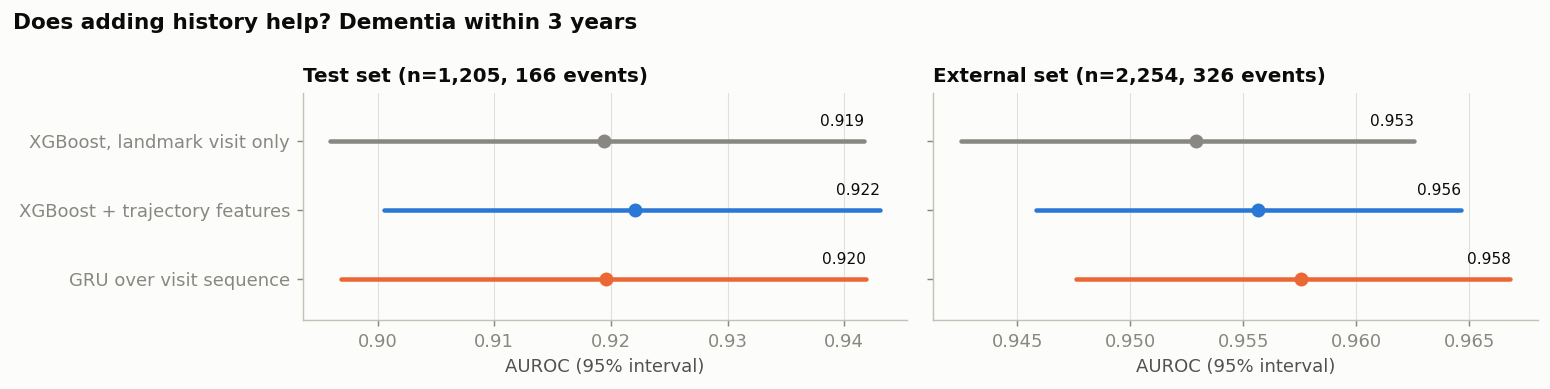
\includegraphics[width=\textwidth]{06_longitudinal.png}
\small
\begin{block}{Visit history}
Landmark visits with $\geq 2$ earlier visits: trajectory features $+0.003$, GRU $+0.000$ to $+0.005$ AUROC.
\end{block}
\end{column}
\begin{column}{0.49\textwidth}
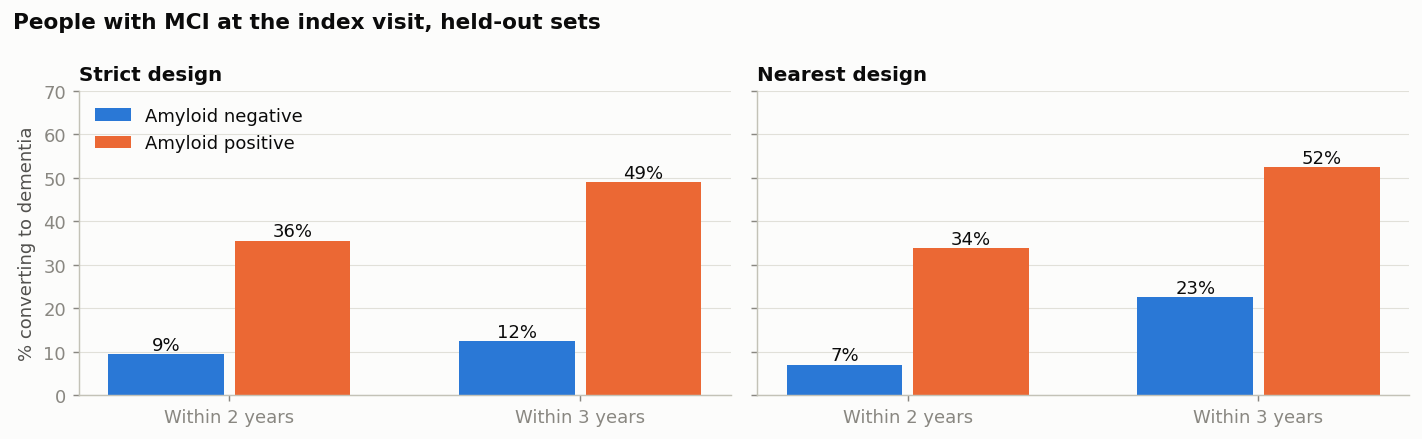
\includegraphics[width=\textwidth]{08_conversion_by_amyloid.png}
\small
\begin{block}{Amyloid and tau PET}
MCI: 34\% of amyloid-positive vs 7\% of negative convert within 2 years. Late fusion: 0.964 vs 0.944 on 243 people (33 events), gain interval $-0.009$ to $+0.066$ includes zero.
\end{block}
\end{column}
\end{columns}
\end{frame}

% ================================================================ 08 PET images
\begin{frame}{08 \textbar\ PET Image Pipeline: From DICOM to SUVR}
\begin{columns}[c]
\begin{column}{0.5\textwidth}
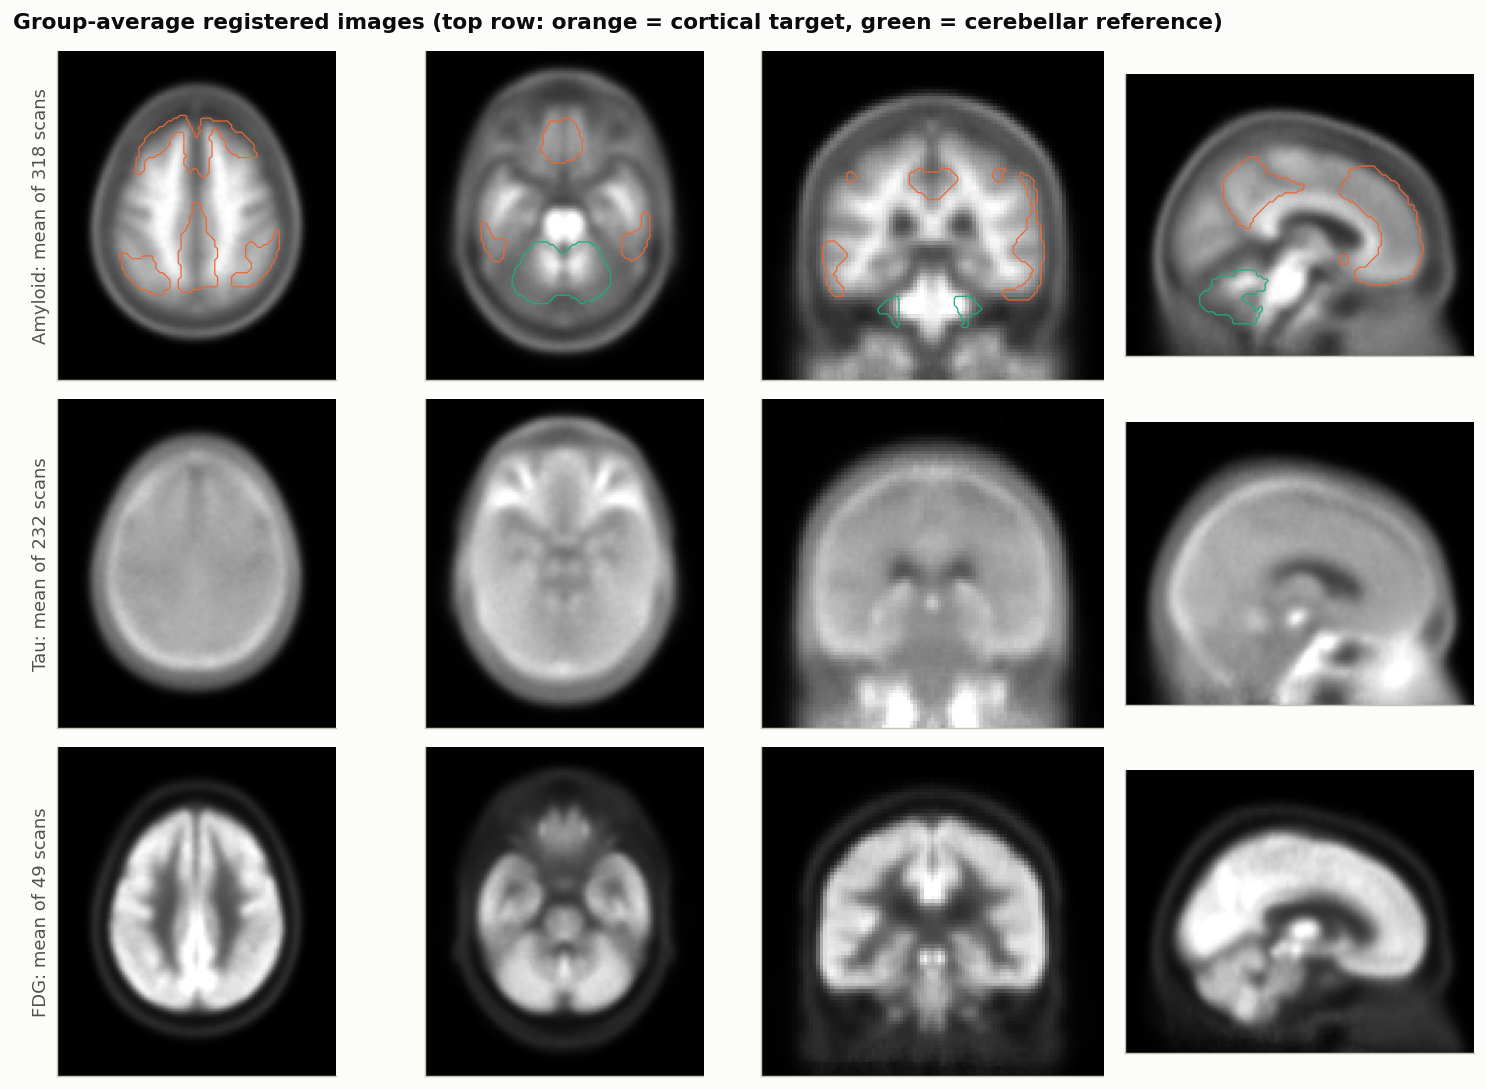
\includegraphics[width=\textwidth]{11_group_average_images.png}
{\tiny Group averages only (318 amyloid, 232 tau, 49 FDG scans).}
\end{column}
\begin{column}{0.48\textwidth}
\small
\begin{enumerate}
\item \textbf{Convert:} 599 dynamic DICOM series $\rightarrow$ static volume, $V = \sum_{k \in \mathcal{W}} d_k V_k / \sum_{k \in \mathcal{W}} d_k$.
\item \textbf{Register:} rigid to MNI152, then 12-parameter affine to a study PET template, Mattes mutual information.
\item \textbf{Quantify:} Centiloid masks, $\text{SUVR} = \bar{V}_{\text{cortex}} / \bar{V}_{\text{cerebellum}}$.
\end{enumerate}
\begin{block}{Validation against the NACC PET core}
Pearson $r = $ \textbf{0.977} over 318 scans (0.96--0.99 per tracer); mean difference $-0.043$.
\end{block}
\end{column}
\end{columns}
\end{frame}

\begin{frame}{3D CNN for amyloid status and Grad-CAM}
\begin{columns}[c]
\begin{column}{0.5\textwidth}
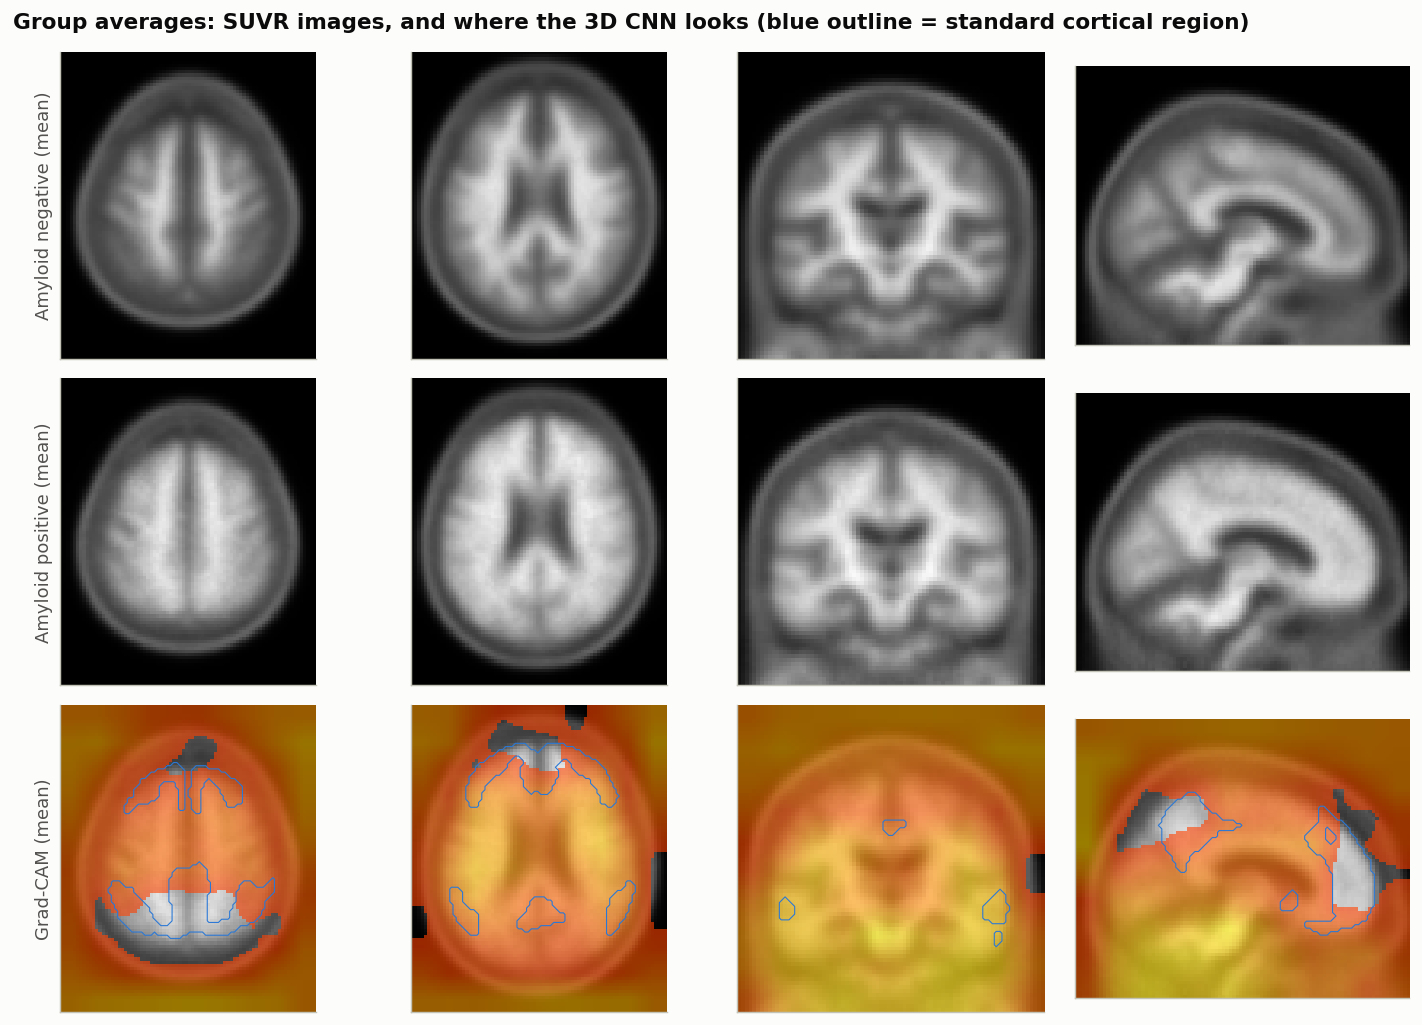
\includegraphics[width=\textwidth]{11_gradcam_mean.png}
\end{column}
\begin{column}{0.48\textwidth}
\small
\begin{tabular}{@{}lc@{}}
\toprule
Method (292 scans, 84 positive) & AUROC \\
\midrule
Cortical SUVR (one number) & \textbf{0.982} \\
Regional logistic model & 0.971 \\
3D CNN (494,917 weights) & 0.960 \\
\bottomrule
\end{tabular}
\vspace{0.4em}
\begin{block}{Interpretation}
The pipeline supports a working image model, but the label is itself derived from cortical SUVR, so one number is hard to beat.
\end{block}
\finding{Limitation}{Grad-CAM was diffuse (1.7\% of top voxels in the cortical region vs 3.8\% by chance), and only 5 imaged people converted, so images were not used to predict dementia.}
\end{column}
\end{columns}
\end{frame}

% ================================================================ 09 validation
\begin{frame}{09 \textbar\ Validation: Calibration, Usefulness, Missing Data}
\begin{columns}[T]
\begin{column}{0.49\textwidth}
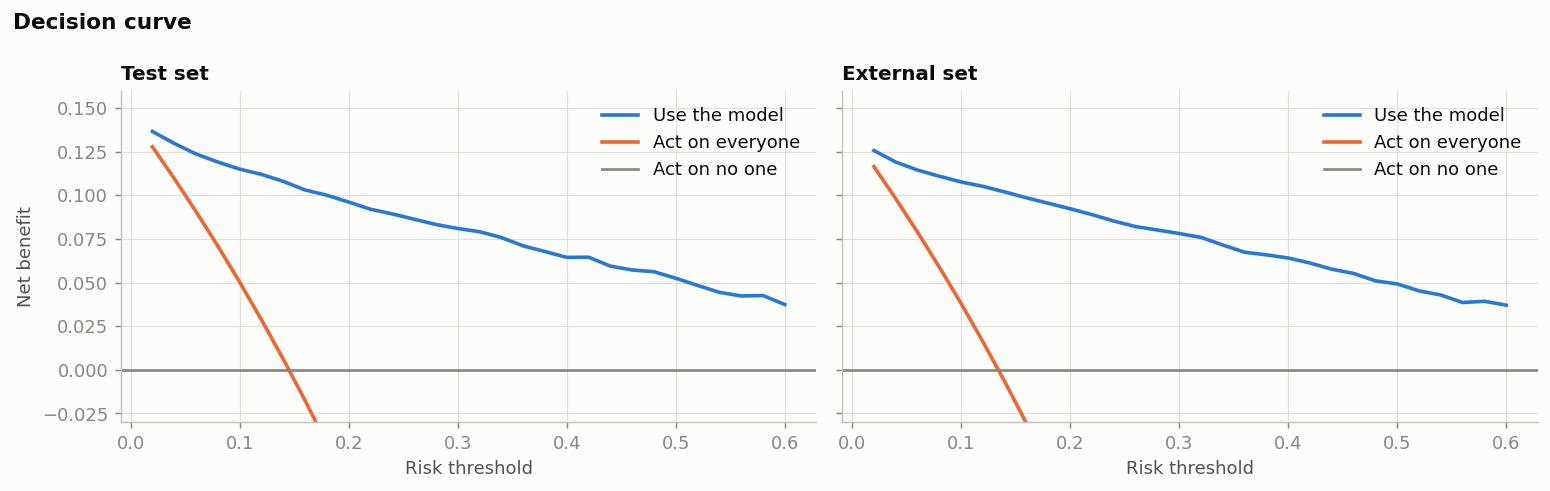
\includegraphics[width=\textwidth]{09_decision_curve.png}
\footnotesize
\begin{itemize}
\item Test: predicted 14.5\% = observed 14.5\%, slope 1.01.
\item Held-out: 15.0\% vs 13.4\%, slope 1.10.
\item At 20\% risk: sensitivity 83\%, specificity 88\%, NPV 97\%.
\item Net benefit above treat-all and treat-none from 2\% to 60\%.
\end{itemize}
\end{column}
\begin{column}{0.49\textwidth}
\footnotesize
\setlength{\tabcolsep}{4pt}
\begin{tabular}{@{}lccc@{}}
\toprule
Brier score & Standard & Dropout & Specialist \\
\midrule
Everything & 0.066 & 0.067 & 0.066 \\
No clinical stage & 0.185 & 0.076 & 0.074 \\
No cognition at all & 0.441 & 0.115 & 0.111 \\
Demographics only & 0.444 & 0.120 & 0.118 \\
\bottomrule
\end{tabular}
\begin{block}{Modality dropout ($p = 0.35$)}
One model stays close to a specialist retrained for each missing pattern; a standard model becomes worse than the base rate.
\end{block}
\end{column}
\end{columns}
\end{frame}

% ================================================================ 10 system
\begin{frame}{10 \textbar\ Research Prototype for Clinicians}
\begin{columns}[c]
\begin{column}{0.42\textwidth}
\centering
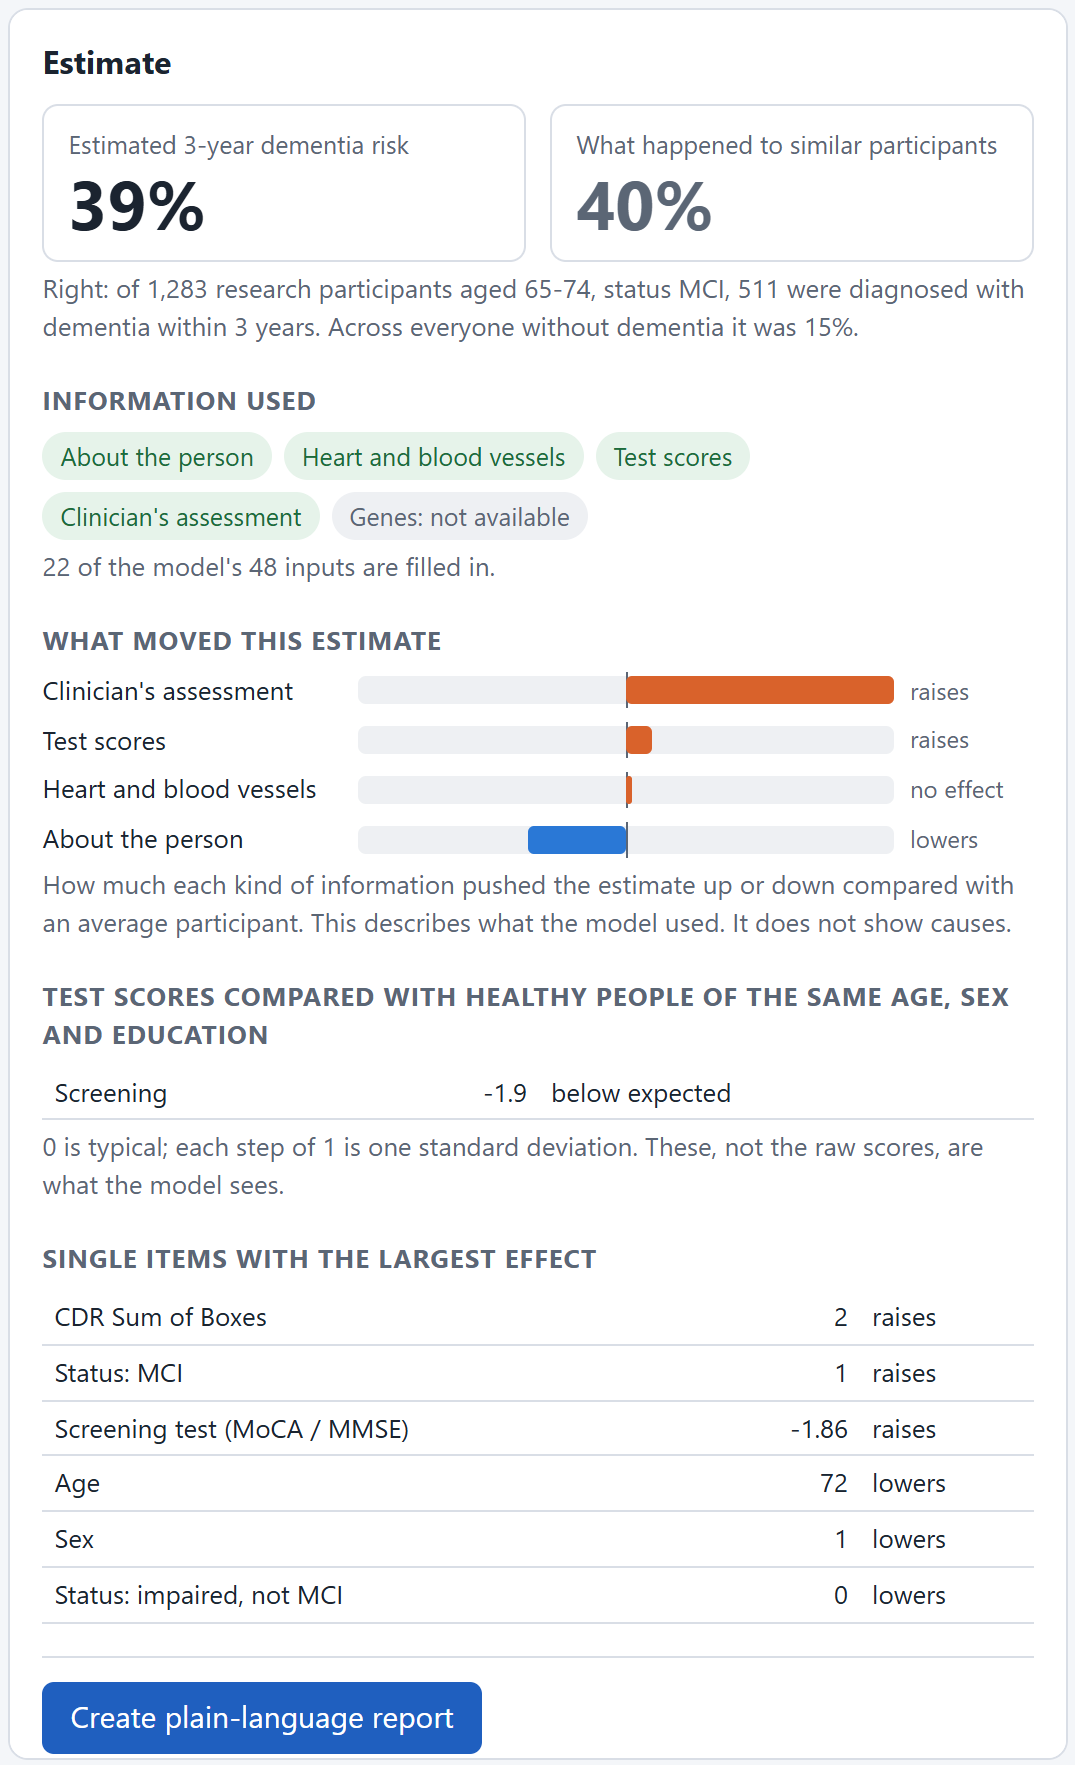
\includegraphics[height=0.8\textheight]{app_estimate.png}
\end{column}
\begin{column}{0.55\textwidth}
\textbf{Example:} 72-year-old woman, 16 years of education, MCI, CDR-SB 2, MoCA 21.\par\medskip
\small
\begin{itemize}
\item FastAPI + React; form generated from the 48 trained features.
\item Risk shown next to the observed rate of similar people, with SHAP by category.
\item Plausibility checks flag contradictory entries.
\item Plain-language report with quoted evidence.
\item 27 of 28 behaviour checks pass; MCI under 65 over-predicted (35\% vs 27\%).
\end{itemize}
\end{column}
\end{columns}
\end{frame}

\begin{frame}{Plain-language report for the same patient}
\begin{columns}[c]
\begin{column}{0.42\textwidth}
\centering
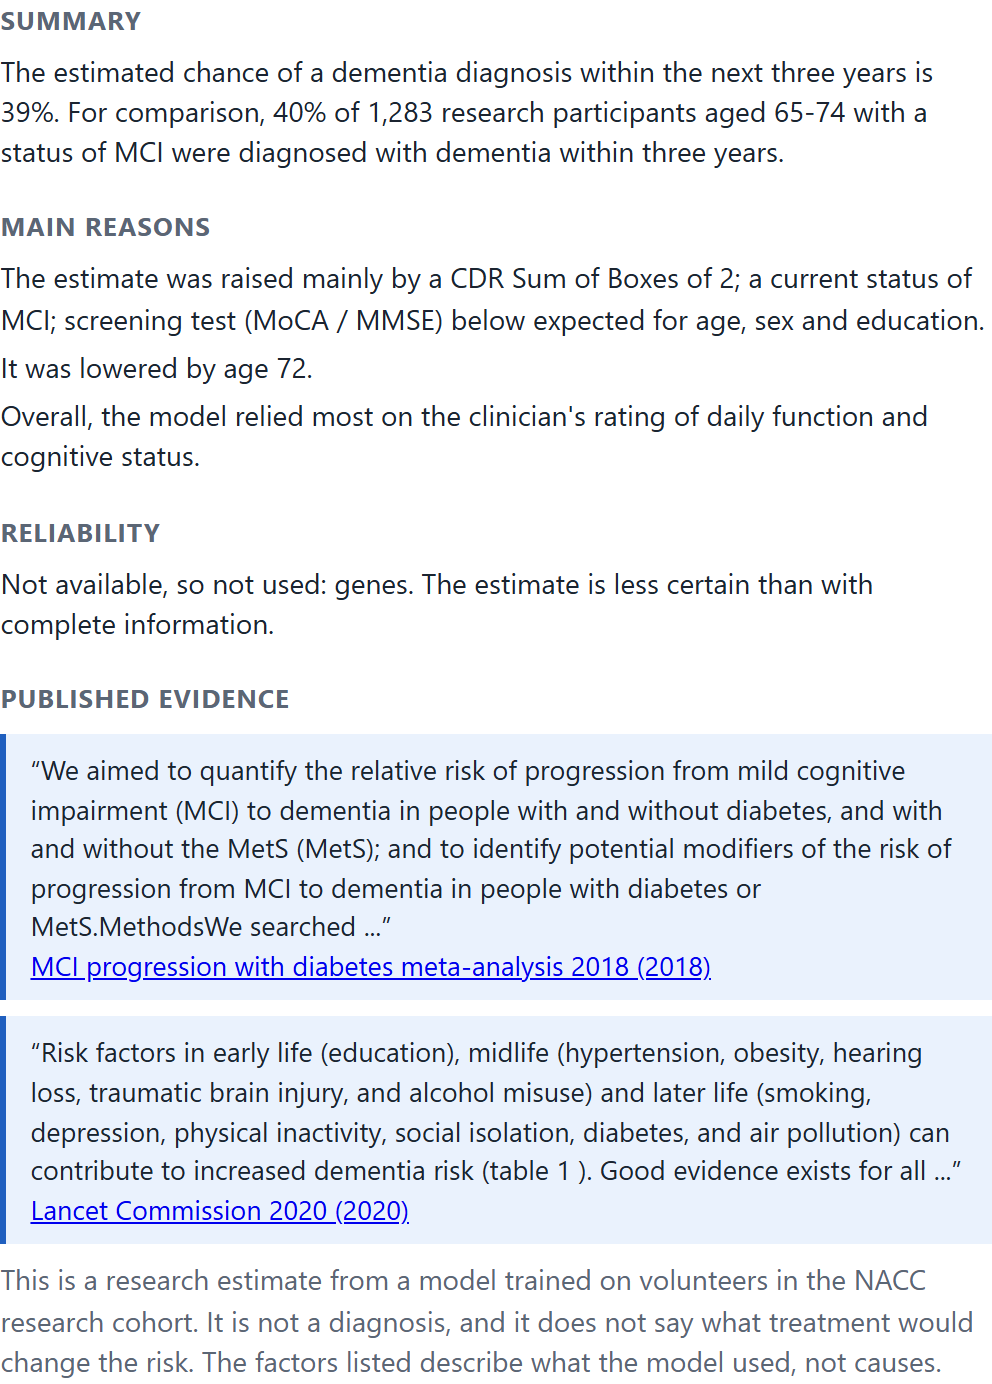
\includegraphics[height=0.8\textheight]{app_report.png}
\end{column}
\begin{column}{0.55\textwidth}
\footnotesize
\begin{enumerate}
\item \textbf{Summary:} risk next to the observed rate of similar people (39\% vs 40\%).
\item \textbf{Main reasons:} largest SHAP contributions in plain words.
\item \textbf{Reliability:} missing categories and plausibility warnings.
\item \textbf{Published evidence:} quoted passages with their source.
\item \textbf{Limits:} fixed statement that it is not a diagnosis.
\end{enumerate}
\begin{block}{Design choice}
Templates are filled with the person's own numbers and evidence is \emph{quoted}, so the report cannot state anything the model or the literature did not provide.
\end{block}
\end{column}
\end{columns}
\end{frame}

\begin{frame}{Evidence assistant (retrieval-augmented generation)}
\centering
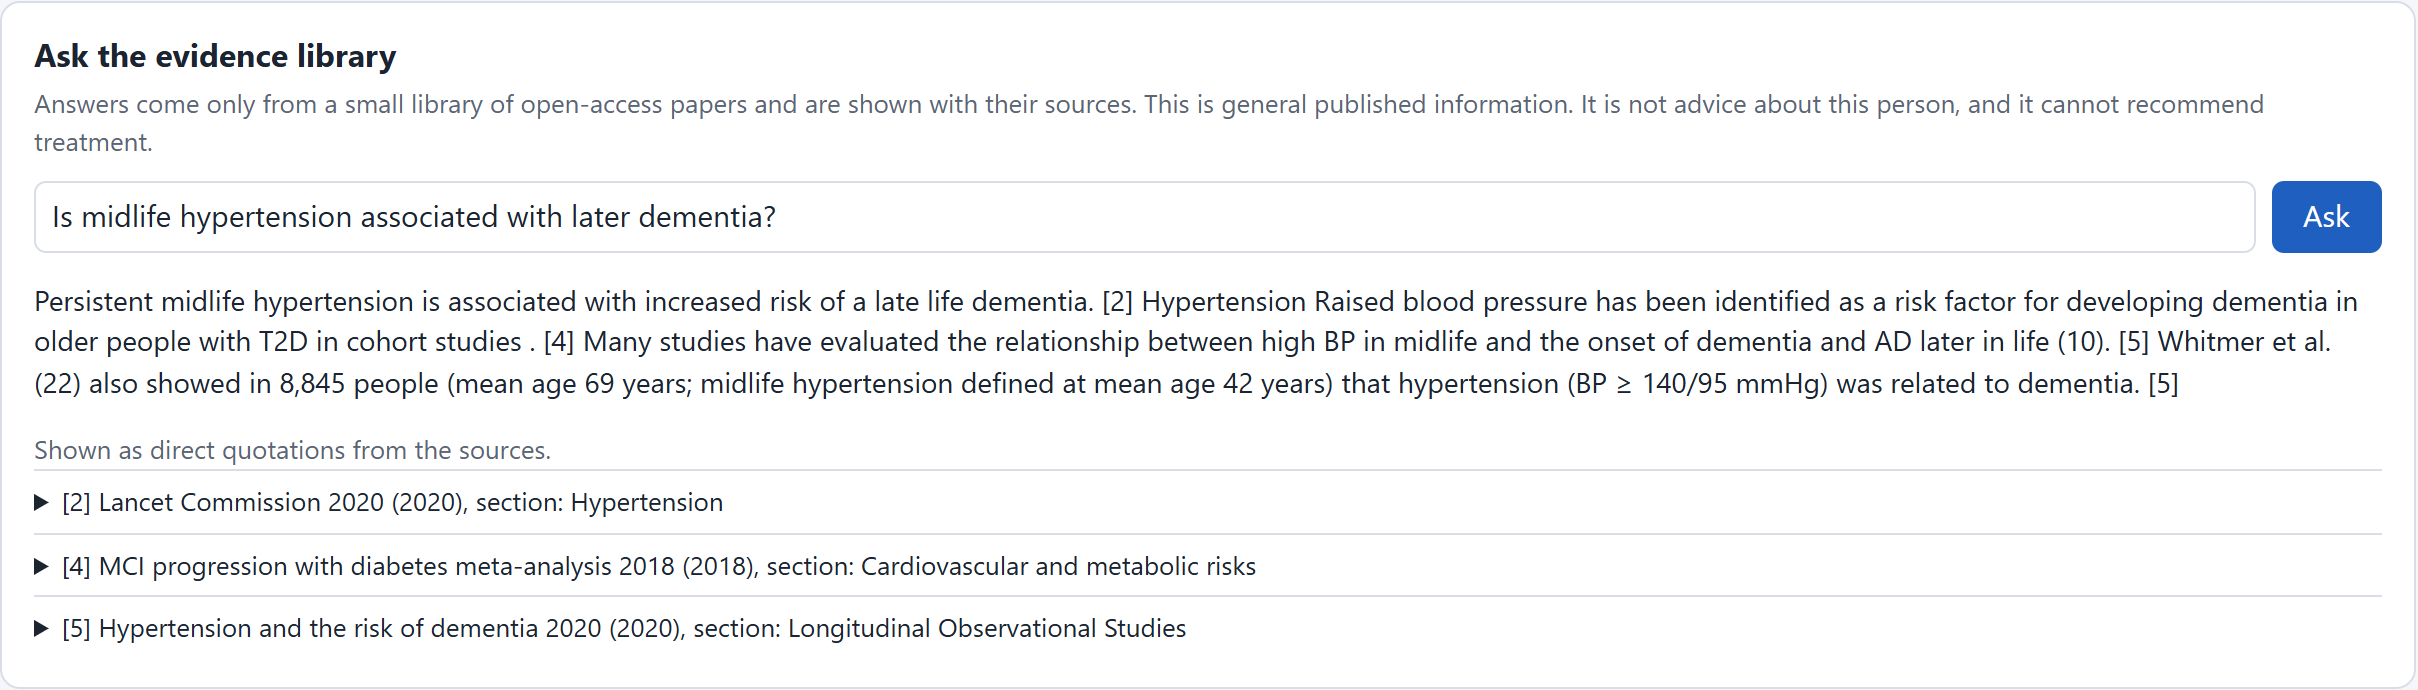
\includegraphics[width=0.86\textwidth]{app_ask.png}
\begin{columns}[T]
\begin{column}{0.48\textwidth}
\small
\[
s_{\text{RRF}}(d) = \frac{1}{60 + \rho_{\text{sem}}(d)} + \frac{1}{60 + \rho_{\text{BM25}}(d)}
\]
MiniLM embeddings + BM25 ($k_1 = 1.5$, $b = 0.75$), merged by rank fusion. Below similarity 0.35 the assistant says the library has no evidence.
\end{column}
\begin{column}{0.48\textwidth}
\footnotesize
\begin{tabular}{@{}lc@{}}
\toprule
Test (11 papers, 447 passages) & Result \\
\midrule
Correct source first: hybrid & 32 / 32 \\
\quad embeddings only / BM25 only & 28 / 31 \\
Personal-advice questions flagged & 8 / 8 \\
Out-of-scope questions declined & 6 / 6 \\
\bottomrule
\end{tabular}
\end{column}
\end{columns}
\end{frame}

% ================================================================ verification
\begin{frame}{11 \textbar\ Independent Verification}
\small
\begin{tabularx}{\textwidth}{@{}lY@{}}
\toprule
Check & Result \\
\midrule
No person or held-out centre in more than one partition & 0 shared \\
Features unchanged when all later visits are deleted & Identical for 1,500 people $\times$ 67 features \\
No PET value newer than the visit that uses it & 0 of 1,481 amyloid, 713 tau \\
Labels recomputed independently & 0 disagreements in 11,403 visits \\
Shuffled labels & AUROC 0.508 (chance) \\
Retrain with a new seed & 0.937 / 0.946 (reported 0.938 / 0.946) \\
\bottomrule
\end{tabularx}
\begin{block}{Errors the checks found and we fixed}
Education and race filled from a \emph{later} visit (0.1\% of people); PET scans matched to visits weeks \emph{before} the scan. After fixing, every model was retrained: results moved only in the third decimal. \textbf{17 of 17 checks pass.}
\end{block}
\end{frame}

% ================================================================ synthesis
\begin{frame}{Synthesis: what each research question found}
\footnotesize
\begin{tabularx}{\textwidth}{@{}p{4.2cm}Y@{}}
\toprule
Research question & Answer and evidence \\
\midrule
RQ1 Prediction accuracy & Dementia 0.94 (0.84 in MCI); decline 0.86 (0.75 in MCI); change regression helps MCI only \\
RQ2 Cardiovascular history & $+0.001$ AUROC once cognition is known; Cox agrees \\
RQ3 Amyloid and tau PET & Strong association, no demonstrable gain with current follow-up \\
RQ4 Deep models / fusion net & No gain over logistic regression or XGBoost; attention uniform \\
RQ5 Earlier visits & $+0.000$ to $+0.005$ AUROC \\
RQ6 Missing categories & Modality dropout keeps calibration close to specialist models \\
RQ7 Explanation and evidence & SHAP, plausibility checks, report with quoted published evidence \\
\bottomrule
\end{tabularx}
\begin{block}{Final takeaway}
How a person is functioning today carries most of the three-year signal; decades of vascular and genetic history leave their trace in that measurement rather than adding to it.
\end{block}
\end{frame}

% ================================================================ limitations
\begin{frame}{Limitations, Future Work and Final Takeaway}
\small
\begin{itemize}
\item Held-out centres are site-level validation within NACC; external and temporal validation on another cohort is the next step.
\item NACC is a research cohort, mostly White and highly educated; about half of eligible people lacked a 3-year outcome (Cox check agrees).
\item Only 24 and 37 cognitively normal converters in test and held-out sets; a dedicated 5- to 10-year model for normal cognition is needed.
\item Richer vascular exposure (repeated blood pressure, treatment, small-vessel imaging) may capture what yes/no history misses.
\item PET registration without MRI, tau not quantified; more follow-up will allow a powered PET test.
\item Evidence library of 11 papers and team-written questions; a curated library and stronger local model would help.
\end{itemize}
\begin{block}{Contribution}
A leakage-free, verified pipeline that measures what each source of information adds, reports results within diagnostic groups, and delivers explainable, evidence-backed estimates.
\end{block}
\end{frame}

{\setbeamertemplate{footline}{}
\begin{frame}[noframenumbering]
\centering
\vspace{2em}
{\color{maroon}\bfseries\Huge Thank you\par}
\vspace{1em}
Questions are welcome.\par
\vspace{2em}
\small Data: National Alzheimer's Coordinating Center (NACC), Freeze 74, used under the NACC data use agreement.\\ All results are aggregates.
\end{frame}}

\end{document}
